%%%%%%%%%%%%%%%%%%%%%%%%%
% Dokumentinformationen %
%%%%%%%%%%%%%%%%%%%%%%%%%
\newcommand{\titleinfo}{Leistungselektronik - Formelsammlung}
\newcommand{\authorname}{\href{mailto:lmazzole@hsr.ch}{L. Mazzoleni}}
%\RequirePackage{luatex85}
%\def\pgfsysdriver{pgfsys-pdftex.def}
\newcommand{\authoremail}{\href{mailto:lmazzole@hsr.ch}{lmazzole@hsr.ch}}
\newcommand{\versioninfo}{$ Entwurf $}

\include{header/header}
\usepackage{nicefrac}
\usepackage{tikz}

%%%%%%%%%%%%%%%%%%%%%%%%%%%%%%%%%%%%%%%%%%%%%%%%%%%%%%%%%%%%%%%%%%%%%%%%%%%%%%%%%%%%%%%%%%%%%%%%

\begin{document}  
\thispagestyle{empty}
\setcounter{page}{0} %Set PageNumber to 0
{\huge README }
\section*{Beschreibung}
Formelsammlung für Leistungselektronik 1 auf Grundlage der Vorlesung HS 16 von Prof. Dr.Jasmin Smajic \newline
Bei Korrekturen oder Ergänzungen wendet euch an einen der Mitwirkenden.
\subsection*{OrCad}
ORCAD Dateien und Simulationen zu den Übungen findet ihr auf OneDrive: \newline
\url{https://1drv.ms/f/s!AigDIY3mrirZhqxYqS0gULPbaWLCfw}\newline
\textbf{Installation}\newline
\begin{itemize}
    \item gehe zu  \textbackslash\textbackslash hsr.ch\textbackslash root\textbackslash alg\textbackslash software\textbackslash Elektrotechnik\textbackslash LeistEl\textbackslash orcad16.6
    \item Rechtsklick auf \" OrcadSetup-starten-Run as administrator \" und \" Run as Administrator \" auswählen
    \item Orcad wird installiert
    \item Nach der Installation dem Hotfix-Link folgen und von dort aus den Hotfix installieren
\end{itemize}

\section*{Modulschlussprüfung}
Prüfungsstoff ist der gesamte LeistEL-Vorlesungsinhalt des HS2016 einschliesslich aller UE + P Lerninhalte.\newline
Als Hilfsmittel für die Modulschlussprüfung sind die Vorlesungen,\newline
UE-Aufgaben und eigenen Praktikumsaufzeichnungen sowie der Taschenrechner erlaubt.

\subsection*{Plan und Lerninhalte}
{\scriptsize 
    \begin{itemize}
        \item Elektronische Schalter (Leistungshalbleiter) und passive Stromrichterkomponenten 
        \item Aufbau und Arbeitsweise netzgeführter Stromrichter 
        \item Wechsel- und Drehstromsteller 
        \item Fremdgeführte Stromrichter
        \item Selbstgeführte Stromrichter
        \item Umrichter
        \item Steuerung und Regelung von Stromrichtern
        \item Einsatz von Stromrichtern in der Energietechnik
        \item Elektromagnetische Verträglichkeit und Netzrückwirkungen
    \end{itemize}
}
\vfill
\section*{Contributors}
\begin{tabular}{ll}
    Luca Mazzoleni& luca.mazzoleni@hsr.ch \\ 
\end{tabular} 

{\scriptsize 
    \section*{License}
    \textbf{Creative Commons BY-NC-SA 3.0}
    
    Sie dürfen:
    \begin{itemize}
        \item Das Werk bzw. den Inhalt vervielfältigen, verbreiten und öffentlich
        zugänglich machen.
        \item Abwandlungen und Bearbeitungen des Werkes bzw. Inhaltes anfertigen.
    \end{itemize}
    Zu den folgenden Bedingungen:
    \begin{itemize}
        \item Namensnennung: Sie müssen den Namen des Autors/Rechteinhabers in der von ihm
        festgelegten Weise nennen.
        \item Keine kommerzielle Nutzung: Dieses Werk bzw. dieser Inhalt darf nicht für
        kommerzielle Zwecke verwendet werden.
        \item  Weitergabe unter gleichen Bedingungen: Wenn Sie das lizenzierte Werk bzw. den
        lizenzierten Inhalt bearbeiten oder in anderer Weise erkennbar als Grundlage
        für eigenes Schaffen verwenden, dürfen Sie die daraufhin neu entstandenen
        Werke bzw. Inhalte nur unter Verwendung von Lizenzbedingungen weitergeben,
        die mit denen dieses Lizenzvertrages identisch oder vergleichbar sind.
    \end{itemize}
    Weitere Details: http://creativecommons.org/licenses/by-nc-sa/3.0/ch/
}
%If we meet some day, 
%and you think this stuff is worth it, you can buy me a beer in return.
\clearpage
\pagenumbering{arabic}% Arabic page numbers (and reset to 1)
\maketitle
\vspace{-2.5cm}
\setcounter{tocdepth}{2}
\tableofcontents
\thispagestyle{empty}
\clearpage
\renewcommand{\arraystretch}{0.6}
\section{Halbleiter}
\begin{itemize}
    \item \textbf{Metallische Leiter:} der Stromtransport wird durch Elektronen erzeugt.
    \item \textbf{Isolatoren:} der Stromtransport wird durch Isolatoren erzeugt.
    \item \textbf{Halbleiter:} die Leitfähigkeit liegt irgendwo zwischen Metallen und Isolatoren.
    \subitem  Die wichtigsten Halbleiter sind  Si, Ge, $CuO_2$ und GaAs 
    \item \textbf{Dotierte Halbleiter:} Durch kontrollierte Verunreinigung (Dotierung) der reinen Halbleiterwerkstoffe kann die Leitfähigkeit wesentlich verändert werden.
\end{itemize}
\subsection{Kristallgitter} 
\begin{minipage}{\linewidth}
        \begin{wrapfigure}{r}{4cm}
            \vspace{-1cm}
            \includegraphics[width=\linewidth]{images/Si-Atom14}  
        \end{wrapfigure}
    Durch die thermische Bewegung der Atomem um ihre Ruhelage im Kristallgitter ist es möglich einige \textbf{Elektronenpaarbindungen} aufzubrechen.\newline
    Auf diese weise ein gelöstes Elektron bewegt sich im Kristallgitter frei und hinterlässt eine \textbf{positiv geladene Lücke im Kristallgitter} (Defektelektron)
\end{minipage}
\newline
\hspace{2cm}
\begin{minipage}{0.3\linewidth}
    \hspace{2cm}
    \includegraphics[width=0.8\linewidth]{images/RGSiT0K}
\end{minipage}
\hspace{2cm}
\begin{minipage}{0.3\linewidth}
    \includegraphics[width=0.8\linewidth]{images/RGSiT300K} 
\end{minipage}
    
\begin{multicols}{2}
\begin{minipage}{\linewidth}
    \subsection{Dotierung}
   Durch eine Dotierung des Halbleitermaterials mit Fremdatomen ist es möglich die Ladungsträgerdichte effizient zu kontrollieren:
\end{minipage}
\includegraphics[width=0.8\linewidth]{images/SiAsDotierung}
\end{multicols}

\begin{multicols}{2}
    \begin{minipage}{\linewidth}
        \vspace{-2cm}
        \subsection{pn-Übergang}
        \subsubsection{Diffusionsstrom}
            Der Diffusionsstrom wird durch den Ladungsträgeraustausch zwischen beiden Halbleitergebieten erzeugt und dadurch verschwinden in der Grenzschicht alle freien Ladungsträger.\\
            Durch die Elektronenwanderung entsteht im n-Teil des Grenzgebiets die \textbf{ortsfeste} Positive Ladung(+). Die eindiffundierten Elektronen erzeugen im p-Teil des Grenzgebiets die \textbf{ortsfeste} negative Ladung (-). Die ortsfesten Ladungen erzeugen das elektrische Feld in der Raumladungszone und dammit auch den Driftstrom.\newline
            Der Driftstrom ist gegen den Diffusionsstrom gerichtet. Sobald die Ströme gleich sind, ist eine stabile Raumladungszone etabliert.   
    \end{minipage}
    
    \includegraphics[width=0.9\linewidth]{images/pnuebergang}
\end{multicols}

\begin{minipage}{\linewidth}
        \subsubsection{pn-Übergang mit äusserer Spannung}
    \begin{wrapfigure}{r}{5cm}
       \vspace{-1cm}
        \includegraphics[width=\linewidth]{images/pnuebergengmitu}
    \end{wrapfigure}
    Die Spannungsquelle ist an den pn-Übergang in \textbf{Sperrrichtung} geschalten.\newline
    Die Spannung U vergrössert die Breite der Raumladungszone. Der Strom kann nicht über den pn-Übergang fliessen.
\end{minipage}
%TODO übersicht silizium germanium selen vor und nachteile
\clearpage
\section{Diode}
Eine Diode besteht aus PN übergängen und ist deswegen ein nichtlineares Element:
\begin{multicols}{2}
     \begin{minipage}{\linewidth}
         \begin{tabular}{ll}
             $ U_{DBR} $    & Durchbruchspanung  \\ 
             $ U_D $        & Diffusionsspannung (0.7V Si)  \\ 
             $ U_F $        & Flussspannung \\ 
             $ U_R $        & Sperrspannung  \\ 
              $ i_F $       & Diffusionsstrom, Strom in Durchlassrichtung  \\ 
              $ i_R $       & Leckstrom, Strom in Sperrichtung \\ 
            \end{tabular} 
        \end{minipage}
        
         \includegraphics[width=0.8\linewidth]{images/kennlinieDiode}
\end{multicols}
\vspace{-1.5cm}
\begin{multicols}{2}
     \begin{minipage}{\linewidth}
         \begin{tabular}{ll}
             $ i_f ,\; u_F $& Durchlassrichtung\\
             $ U_{T0} $& Schwellenspannung\\
             $ r_f= \dfrac{\diff U_F}{\diff i_F} $& Differenzieller Durchlasswiderstand\\
            \end{tabular}       
    \end{minipage}
        
        \includegraphics[width=0.4\linewidth]{images/dDiodeKennlinie}
\end{multicols}
\vspace{-1.5cm}
\subsection{Ersatzschaltbild}
\begin{multicols}{4}
    \begin{minipage}{\linewidth}
        \textbf{Reale Diode} \raggedright \newline\newline
        \includegraphics[width=0.7\linewidth]{images/realeDiode}
    \end{minipage}
    
    \begin{minipage}{\linewidth}
        \textbf{Ideale Diode ($ D_1 $)} \raggedright \newline\newline
        \includegraphics[width=0.7\linewidth]{images/idealeDiode}
    \end{minipage}
    
    \begin{minipage}{\linewidth}
        \textbf{Diode $ D_1 $ mit der Schwellenspannung $  D_2 $} \raggedright
        \includegraphics[width=0.6\linewidth]{images/idealeDiodeSP}
    \end{minipage}
    
    \begin{minipage}{\linewidth}
        \textbf{Diode $ D_2 $ mit dem Durchlasswiderstand($ D_3 $)} \raggedright
        \includegraphics[width=0.6\linewidth]{images/idealeDiodeSPR}    
    \end{minipage}                       
\end{multicols}
\begin{multicols}{2}
\subsection{Grundformeln}
\begin{tabular}{ll}
    \textbf{Flussspannung}&\[ u_F = U_{T0} + i_F \cdot r_F \]\\
    \textbf{Momentanleistung}&\[ p(t)=u_F(t)\cdot i_F(t) \]\\
    \textbf{Verlustleistung}&\[ P_v=U_{TO}\cdot I_{FAV}+r_F\cdot I_{FRMS}^2 \]\\
    $ I_{FAV}$ & \qquad arithmetische Mittelwert von $ i_F $\\
    $ I_{FRMS} $ & \qquad Effektivwert von $ i_F $\\    
\end{tabular}

\hspace{1cm}\includegraphics[width=0.6\linewidth]{images/ESBDiode} 
\end{multicols}

\subsection{Schaltverhalten und Schaltverluste}
    \begin{minipage}{0.7\linewidth}
        \raggedright
        \textbf{Durchlassverzug:}\newline
        freie Ladungsträger müssen zuerst die Ladungsfrei Zone "füllen"\newline\newline
        \textbf{Sperrverzug}\newline
        freie Ladungsträge müssen zuerst das Gebiet des pn-Überganges freiräumen\newline\newline
        Diese Erscheinungen sind wichtig bei  $\nicefrac{\diff u}{\diff t} > 100 \nicefrac{V}{\mu s} \; und \; \nicefrac{\diff i}{\diff t} > 10 \nicefrac{A}{\mu s} $
        \begin{tabular}{ll}
            $ I_{RM} $&Maximalwert des Rückstroms\\
            $ U_{RM} $&Maximalwert der Rückspannung\\
        \end{tabular}
    \end{minipage}   
    \begin{minipage}{0.3\linewidth}
        \vspace{-0.8cm}
        \raggedleft
            \includegraphics[width=\linewidth]{images/idealeDiodeSS}           
            \includegraphics[width=\linewidth]{images/realeDiodeSS}
    \end{minipage}
\clearpage

\section{Transistor}
\vspace{-0.2cm}
\subsection{Bipolarer Transistor}
\vspace{-0.2cm}
\subsubsection{Wirkungsprinzip}
Ein Bipolartransistor besteht aus drei dünnen dotierten Halbleiterschichten, d.h. aus zwei pn-Übergängen. Gemäss der Reihenfolge und dem Dotierungstyp der Schichtung werden Bipolartransistoren in npn- und pnp-Typen unterteilt.\newline Als Leistungstransistoren werden überwiegend npn-Transistoren in der Emitter-Schaltung verwendet\newline
\hspace*{2cm}
\begin{tabular}{ccc}
     \textbf{Wirkungsprinzip}&\textbf{Aufbau}&\textbf{Schaltzeichen}\\
     \includegraphics[width=0.35\linewidth]{images/npnTransistor}&
     \includegraphics[width=0.15\linewidth]{images/aufbautransnpn}&
     \includegraphics[width=0.25\linewidth]{images/esbtransnpn} \\
\end{tabular}

\subsubsection{Schaltverhalten}
\begin{minipage}{0.6\linewidth}
    \begin{wrapfigure}{r}{4cm}
        \includegraphics[width=\linewidth]{images/npnTransemitter}
    \end{wrapfigure}
    \raggedright
    \textbf{Im Sättigungsbreich} ist der Basisstrom so gross, dass sich in der Basiszone mehr Ladungsträger befinden als für den Kollektorstrom nötig ist.\newline\newline
    Die beiden pn-Übergänge sind in die Durchlassrichtung polarisiert.\newline
    $ U_{BE}>U_{CE} $ und $ U_{BC}>0 $\newline\newline
    Im Verstärkungsbereich gilt: $ \beta = \dfrac{I_C}{I_B} $\newline \newline
    \textbf{Im Schaltbetrieb} werden die Arbeitspunkte \textbf{I} (vorwärts sperrend) und \textbf{III} (Durchlassbetrieb -Sättigung) verwendet.
\end{minipage}
\begin{minipage}{0.4\linewidth}
    \includegraphics[width=0.8\linewidth]{images/npnTranskennlinie}
\end{minipage}
\subsubsection{Kennwerte}
\begin{minipage}{0.5\linewidth}
	\renewcommand{\arraystretch}{1.2}
\begin{tabular}{l p{7cm}} 
    \textbf{$ U_{CES} $}&\textbf{Kollektor-Emitter-Sperrspannung}\\
    &Der höchstzulässige Wert der $ U_{CES} $ bei Ansteuerung mit einer negativen $ U_{BE} $\\
    \textbf{$ U_{CE0} $}&\textbf{Kollektor-Emitter-Sperrspannung}\\%RICHTIG??
    & Der höchstzulässige Wert der $ U_{CE} $ bei offenem Basisanschluss\\
    \textbf{$ I_{CAVM} $}&\textbf{Kollektor-Dauergrenzstrom}\\
    &\mbox{Der höchstzulässige Wert des Gleichstrom-} \mbox{Mittelwerts bei vorgegebener Temperatur}\\
    \textbf{$ I_{CRM} $}&\textbf{periodischer Kollektor-Spitzenstrom}\\
    &\mbox{Der höchstzulässige Wert eines Pulsstromes} \mbox{mit angegebener Periodendauer und Einschaltdauer}\\
\end{tabular}
\end{minipage}
\begin{minipage}{0.5\linewidth}
    \includegraphics[width=\linewidth]{images/npnTransESV}
\end{minipage}

\begin{minipage}{0.5\linewidth}
    \subsubsection{Verluste}
    \begin{itemize}
        \item Einschaltverluste
        \item Ausschaltverluste
        \item Durchlassverluste
        \item Sperrverluste
    \end{itemize}
\end{minipage}
\begin{minipage}{0.5\linewidth}
    \hspace{0.5cm}\includegraphics[width=\linewidth]{images/npnTransVerluste}
\end{minipage}
\clearpage

\vspace*{-1cm}
\subsection{Darlington-Transistoren}
%\begin{wrapfigure}{r}{2cm}
%    \includegraphics[width=\linewidth]{images/darlingtonSymbol}
%\end{wrapfigure}
Der Stromverstärkungsfaktor der Leistungstransistoren ist relativ klein. Deswegen ist ein starker Basisstrom für diese Transistoren notwendig. Ein Darlington-Transistor löst dieses Problem.\\[0.1cm]
\begin{minipage}{0.6\linewidth}
    \subsubsection{Formeln}
    \vspace{-0.2cm}
    $ \beta = \text{Kleinsignalverstärkung}$\newline
    $B = \text{Grosssignalverstärkung}$
    \vspace{-0.2cm}
    \[ \beta_1 = \dfrac{i_{C1}}{i_{B1}}, \qquad \beta_2 = \dfrac{i_{C2}}{i_{B2}} \]    
    \[ i_{E1} = i_{C1}+i_{B1}=(1+\beta_1)i_{B1} = i_{B2} \]
    \[ i_{C2} = \beta_2 i_{B2} = \beta_2 i_{E1} = \beta_2 (1 + \beta_1)i_{B1}=\beta_{ges}i_{B1} \]
    \[ \beta_{ges} = \beta_2(1 + \beta_1) \approx \beta_1 \beta_2 \]    
\end{minipage}
\begin{minipage}{0.3\linewidth}
    \subsubsection{Aufbau}
    \includegraphics[width=4cm]{images/darlingtonaufbau}
     \includegraphics[width=1.5cm]{images/darlingtonSymbol}
\end{minipage}
 \vspace{-0.2cm}
\subsubsection{Vor und Nachteile}
\vspace{-0.5cm}
\begin{multicols}{2}
    \begin{minipage}{\linewidth}
        \begin{itemize}
            \item [+] Gleichbleibender Platzbedarf
            \item [+] höhere Stromverstärkung
            \item [+] $ B \approx B_1 \cdot B_2 $ im Bereich <1000 
            \item [+] $ \beta \approx \beta_1 \cdot \beta_2 $ im Bereich <50'000
        \end{itemize}
    \end{minipage}
    
    \begin{minipage}{1.2\linewidth}
        \begin{itemize}
            \item [-] grosse Phasenverschiebung
            \item [-] für Hochfrequenzanwendungen ungeeignet
            \item [-] langsame Schaltzeiten
            \item [-] doppelte Basis-Emitter-Spannung
        \end{itemize}
    \end{minipage}
\end{multicols}
Für effiziente Schaltanwendungen eignen sich Darlingtontransistoren wegen diesen Nachteilen kaum.
 \vspace{-0.2cm}
\subsection{MOSFET}
\begin{wrapfigure}{r}{7cm}
    \vspace{-1cm}
    \includegraphics[width=\linewidth]{images/mosfetprinz}
    \newline
    \includegraphics[width=\linewidth]{images/mosfetprak}
\end{wrapfigure}
Die elektrische Leitfähigkeit des Substrats ist durch ein el. Feld gesteuert. Das el. Feld ruft im Substrat eine Influenzladung hervor.\newline
Die Gate-Elektrode ist durch ein Metalloxid vom Substrat isoliert.\\[0.3cm]
\begin{tabular}{ll}
    S = Source & D = Drain\\
    G = Gate & B = Bulk (Substrat)\\
\end{tabular}\\[0.3cm]
$ U_{DS} $ ist positiv damit ist der rechte pn-Übergang in Sperrrichtung gepolt. Deswegen kann kein Strom in beide Richtungen fliessen.\newline
$ \rightarrow $ Der Transistor ist selbstsperrend.\newline
\danger~Sobald eine positive Spannung zwischen $ G $ und $ S $ angelegt ist, entsteht ein leitfähiger n-Kanal und damit auch ein Strom vom \\D- zum S-Anschluss.
 \vspace{-0.2cm}
\subsection{IGBT}
Der IGBT setzt such aus einem Bipolartransistor $ T_2 $ und einem MOSFET $ T_1 $ zusammen.\newline
    n- ist eine schwach dotierte Zone, welche zur Erhöhung der Spannungsfestigkeit verwendet wird.
\begin{center}
  \includegraphics[width=0.7\linewidth]{images/IGBTaufbau}
  \includegraphics[width=0.25\linewidth]{images/IGBTkennlinie}
\end{center}
\vspace{-0.5cm}
\subsubsection{Eigenschaften}
\begin{multicols}{2}
    \begin{itemize}
        \item \mbox{Über die Kollektor-Emitter-Strecke fällt} \newline \mbox{mindestens die Schleusenspannung ab}
        \item Kleine Durchlassverluste bei hohen Strömen
        \item In Rückwärtsrichtung nur begrenzt sperrfähig
        \item Grosse Sperrverluste vorallem beim Abschalten
    \end{itemize}
\end{multicols}
\clearpage

\subsection{Transistoren im Vergleich}
\includegraphics[width=\linewidth]{images/transdiff}
%\begin{tabular}{lccc}
%    &\textbf{Darlington-Transistor}&\textbf{MOSFET}&\textbf{IGBT}\\
%    Schaltsymbol&
%    \includegraphics[width=1cm]{images/darlingtonSymbol}&
%    \includegraphics[width=2cm]{images/MOSFETSymbol}&
%    \includegraphics[width=1cm]{images/IGBTSymbol}\\
%    
%    Schichtaufbau&
%    \includegraphics[width=1cm]{images/darlingtonSchicht}&
%    \includegraphics[width=1cm]{images/MOSFETSchicht}&
%    \includegraphics[width=1cm]{images/IGBTSchicht}\\
%    
%    &&&\\
%    &&&\\
%    &&&\\
%    &&&\\
%    &&&\\
%    &&&\\    
%\end{tabular}

%=========================================
\clearpage
\begin{minipage}{0.7\linewidth}
\section{Thyristoren}
Ein Thyristor besteht aus vier Halbleiterschichten d.h. aus drei pn-Übergängen \newline
Thyristoren sind einschaltbare Bauelemente.\newline
Thyristoren sind  \"{}einschaltbare Dioden\"{}. Thyristoren werden mit dem \newline Zündimpuls der zwischen Gate (G) und Kathode (K) kurzzeitig anliegt durchgeschaltet.
\end{minipage}
\begin{minipage}{0.3\linewidth}
     \hspace{1cm}\includegraphics[width=0.5\linewidth]{images/thyraufbau}
\end{minipage}
\includegraphics[width=0.15\linewidth]{images/thyrESB}
\includegraphics[width=0.4\linewidth]{images/thyrKennlinie}
\includegraphics[width=0.45\linewidth]{images/thyrSchaltung}
\subsection{Thermische Ersatzschaltung}

\begin{multicols}{3}
    \begin{minipage}{\linewidth}
        \textbf{Thermische Kenngrösse}\newline
        Wärmeleistung P [W]\newline
        Temperaturunterschied $ \vartheta $ [K]\newline
        Wärmewiderstand $ R_{th} $ [${K}/{W}$]\newline
        \textbf{Elektrische Kenngrösse}\newline
        Strom I  [A]\newline
        Spannung [V]\newline
        Widerstand [$\nicefrac{V}{A}, \Omega$]\newline
    \end{minipage}
	\begin{minipage}{\linewidth}
		\subsubsection{Thyristor ohne Kühlung}
		\includegraphics[width=\linewidth]{images/thyrOK}
		\[ \vartheta_{vJ}-\vartheta_U=P \cdot (R_{th\; JG}+R_{th\; GU}) \]		
	\end{minipage}
	\begin{minipage}{\linewidth}
		\vspace{0.2cm}
		\subsubsection{Thyrisor mit Kühlung}
		\includegraphics[width=\linewidth]{images/thyrMK}
		\[ \vartheta_{vJ}-\vartheta_U=P \cdot (R_{th\; JG}+R_{th\; GK}+R_{th\; KU}) \]	
        \[ R_{th \; KU}=\dfrac{\Delta \vartheta}{P} \]
	\end{minipage}
\end{multicols}
\vspace{-1.5cm}
\textbf{Beispiel Schaltverluste bei B2C}\newline
\begin{tabular}{ll}
    Spitzenwert des Thyristorstromes&
    $\widehat{I}_{R} = \frac{\widehat{U}_{2}}{R}$\\
    \\
    
    Mittelwert des Thyristorstromes &
    $I_{T AV} = \frac{1}{2\pi}\int\limits_{\alpha}^{\pi}I_{Rm} \cdot sin(\beta)\diff\beta= \frac{\widehat{I}_{R}}{2\pi} \cdot (1+cos(\alpha))$\\

    Effektivwert des Thyristorstromes &
    $I_{T RMS} = \sqrt{\frac{I_{RM}^2}{2\pi}\int\limits_{\alpha}^{\pi}sin^2(\beta)\diff\beta}= \frac{\widehat{I}_{R}}{2}\sqrt{\frac{\pi - \alpha}{\pi}+\frac{sin(2\alpha)}{2\pi}}$\\

    momentane Verlustleistung:&
    $p(t) = u_{T}(t) \cdot i_{T}(t)$\\
    Mittelwert der Verlustleistung: &
    $P_{T} = \frac{1}{T}\int\limits_{0}^{T}u_{T}(t) \cdot i_{T}(t)\diff t = U_{T0} \cdot \frac{1}{T}\int\limits_{0}^{T}i_{T}(t)\diff t+r_{T} \cdot \frac{1}{T}\int\limits_{0}^{T}i_{T}^2(t)\diff t$\\
    \\
    & $P_{T} = U_{T0} \cdot I_{T AV} + r_{T} \cdot I_{T RMS}^2$\\[0.3cm]
\end{tabular}

 $I_{T AV}$ ist der Mittelwert und $I_{T RMS}$ der Effektivwert des Thyristorstroms\\[0.2cm]
\textbf{Der Wert für $U_{T0}$ kann aus dem Datenblatt des Thyristors herausgelesen werden.}\\[0.2cm]

\begin{minipage}{0.5\linewidth}
    \subsection{Abschaltbarer Thyristor}
    \begin{minipage}{0.7\linewidth}        
        \textbf{(GTO = Gate-Turn-Off)}\newline
        Der GTO schaltet aus, wenn ein ausreichend hoher negativer Gate-Strom \newline auftritt.\newline
        Amplitude des Gate-Stromes muss 20\% bis 30\% des abzuschaltenden GTO-Stromes betragen.
    \end{minipage}
    \begin{minipage}{0.2\linewidth}
        \includegraphics[width=\linewidth]{images/GTOSymbol}
    \end{minipage}    
\end{minipage}
\begin{minipage}{0.5\linewidth}
    \subsection{IGCT}
    	        \begin{wrapfigure}{r}{1.5cm}
    	        	\vspace{-1cm}
    	\includegraphics[width=\linewidth]{images/IGCTSymbol}
    \end{wrapfigure} 
    \begin{minipage}{\linewidth}
        \textbf{Integrated Gate-Commutated Thyristor}\\
        IGCT sind die Weiterentwicklung der GTO.\newline
        Sie werden hauptsächlich für Mittel\-spannungs\-umrichter eingesetzt.
    \end{minipage}
\end{minipage}
\clearpage

\section{Stromrichterschaltung}
\subsection{Gruppierung}
\subsubsection{nach Steuerung}
\begin{itemize}
    \item Ungesteuerte Stromrichter:
        \subitem Das Verhältniss von Eingans- zu Ausgangsspannung wird durch die Stromrichterschaltung festzgesetzt
    \item Gesteuerte Stromrichter
        \subitem Das Verhältniss von Eingans- zu Ausgangsspannung wird durch Steuereingriff am Halbleiterschalter verändert. 
\end{itemize}

\subsubsection{nach Führung}
\href{https://de.wikipedia.org/wiki/Kommutierung}{Kommuntierung WIKI}\newline
\begin{minipage}{0.6\linewidth}
Bzw nach der Herlkunft der Kommutierungsspannung.\newline
Kommutierung bedeutet die Wechslung des Stromflusses von einem HL-Ventil auf ein anderes.
\begin{itemize}
    \item Netzgeführte Schaltung
        \subitem Kommutierungsspannung vom Netzwerk
    \item Lastgeführte Schaltung
        \subitem Kommuntierungsspannung wird durch Lastkreis (zb Synchronmotor) gesteuert
    \item Selbstgeführte Schalung
        \subitem Kommutierungsspannung wird selbst erzeugt
\end{itemize}
\end{minipage}
\begin{minipage}{0.4\linewidth}
    \includegraphics[width=\linewidth]{images/StromrichterKennzeichnung}\newline
\end{minipage}

\subsection{Kennzeichnung}
\includegraphics[width=0.9\linewidth]{images/SRKennzeichnung}\newline
\href{https://de.wikipedia.org/wiki/Gleichrichter}{Gleichrichter WIKI}

%===================================================================
\clearpage
    \section{Ungesteuerter Gleichrichter}
\subsection{M1U}
\vspace{-0.5cm}
\begin{minipage}{0.4\linewidth}
    \includegraphics[width=\linewidth]{images/PrakUGM1}
\end{minipage}
\begin{minipage}{0.3\linewidth}
    \centering
   \includegraphics[width=0.7\linewidth]{images/PrakUGM1Kl1}
   \includegraphics[width=0.7\linewidth]{images/PrakUGM1Kl2}
\end{minipage}
\begin{minipage}{0.3\linewidth}
    \includegraphics[width=\linewidth]{images/UGM1OW} 
\end{minipage}
\newline

%\includegraphics[width=0.4\linewidth]{images/UGRM1U}
%\includegraphics[width=0.2\linewidth]{images/UGRM1US} \newline
\vspace{-0.3cm}
Die Diode wird als ideal betrachtet $ \rightarrow $ keine Schwellenspannung oder Innenwiderstand
	\renewcommand{\arraystretch}{1}
	\vspace{-0.2cm}
\begin{longtable}{| p{.3\textwidth} | p{.40\textwidth} | p{.25\textwidth} |} 
    \hline
    \textbf{Grundgleichungen}&
    \vspace{-0.5cm}
    \[ U_2 = U_D + U_R \]
    \[ U_R = I_2 \cdot R\]
    \[ U_{OUT} = \dfrac{\widehat{U}}{\pi}\]\vspace{-1cm}&
    \textbf{Durchlassrichtung}\newline
    $ 0 < \omega t < \pi $\newline
    $U_2 = U_R \qquad U_D = 0$\newline

    \textbf{Sperrichtung}\newline
    $ \pi < \omega t < 2\pi $\newline
    $ U_2=U_D \qquad U_R = 0 $\newline
    \\
    \hline
    
    \textbf{Wirkleistung der Last R}&
    \vspace{-0.5cm}
    \[ P=\frac{1}{2\pi} \int_{0}^{2\pi} p(\alpha) d\alpha = \dfrac{U_{R\;RMS}^2}{R} \] \vspace{-0.5cm}&
    \\ \hline
\end{longtable}
%
%Leistung = Momentanleistung des Sormes x momentanleistung der Spannung\\
%Leistung = Leistung bei trafoseite messen 1harm des stroms phasenverschiebung -> u i cos(phi) fourierreihen..
%Leistung = Irav* U1harm  
\vspace{-0.3cm}
\textbf{Oberwellen}\\[0.2cm]
\vspace{-1cm}
\begin{figure}[h]
	\begin{subfigure}[t]{0.5\linewidth}
		\includegraphics[width=\linewidth]{images/M1UR}
		\subcaption{R}
	\end{subfigure}
\begin{subfigure}[t]{0.5\linewidth}
	    \includegraphics[width=\linewidth]{images/M1URL}
	    \subcaption{R + L}
\end{subfigure}
\begin{subfigure}[t]{0.5\linewidth}
	    \includegraphics[width=\linewidth]{images/M1URLD}
	    \subcaption{R + L+ Freilaufdiode}
\end{subfigure}
\begin{subfigure}[t]{0.24\linewidth}
    \includegraphics[width=\linewidth]{images/M1URLKl}
    \subcaption{R + L Kennlinie}
\end{subfigure}
\begin{subfigure}[t]{0.25\linewidth}
    \includegraphics[width=\linewidth]{images/M1URCKl}
    \subcaption{R + C Kennlinie}
\end{subfigure}
\end{figure}
\vspace{-0.8cm}
\subsubsection{Rechnungsbeispiel}
\textbf{Übung 2 - Gleichrichter M1U}\newline
\renewcommand{\arraystretch}{1.3}
\begin{tabular}{ p{.3\textwidth}  p{.40\textwidth}  p{.25\textwidth}}
    Ausgangslage:&
    $ U_2= U_{2m}\cdot sin(2\pi ft)$&
    \\
    Mittelwert Spannung: &
    $ U_{R \; AV}= \frac{1}{2 \pi} \int\limits_{0}^{\pi} U_{2m}\cdot sin(\alpha)\diff\alpha=\frac{U_{2m}}{\pi} $ &
    $ \alpha=\omega t $
    \\
    
    Effektivwert Spannung:   &
    $ U_{R \; RMS}= \sqrt{\frac{1}{2 \pi}\int\limits_{0}^{\pi} U_{2m}^2\cdot sin(\alpha)^2\diff\alpha} = \frac{U_{2m}}{2} $ &
    \\ 
    
    Mittelwert Strom: &
    $ I_{R \; AV}=\frac{U_{R \; AV}}{R_L}= \frac{1}{\pi}\frac{U_{2m}}{R}= \frac{1}{\pi} I_{2m} $ &
    \\
    
    Effektivwert Strom: &
    $ I_{R \; RMS}=\frac{U_{R \; RMS}}{R}= \frac{U_{2m}}{2R}= \frac{I_{2m}}{2} $ &
    \\
    
    Wirkleistung R: &
    $ P= \frac{1}{2\pi}\int\limits_{0}^{\pi}\frac{u_R^2(\alpha)}{R} \diff \alpha = \frac{U_{R \; RMS}^2}{R}=\frac{1}{R}\frac{U_{2m}^2}{4} $&
    \\
    
    Wirkleistung Sekundärseite: &
    $P_2 = U_2 \cdot (I_2)_1 \cdot cos(\varphi)_1 = \frac{U_{2m}}{\sqrt{2}} \cdot \frac{b_1}{\sqrt{2} \cdot R}$&
    \\
\end{tabular}\vspace*{-1cm}
\renewcommand{\arraystretch}{1}

%===================================================================
\clearpage

\subsection{B2U}
\begin{minipage}{0.4\textwidth}
    \includegraphics[width=\linewidth]{images/PrakUGB2}
\end{minipage}
\begin{minipage}{0.25\linewidth}
    \centering
    \includegraphics[width=0.9\linewidth]{images/PrakUGB2Kl1}
    \includegraphics[width=0.9\linewidth]{images/PrakUGB2Kl2}
\end{minipage}
\begin{minipage}{0.35\linewidth}
    \includegraphics[width=\linewidth]{images/UGB2OW}
\end{minipage}\newline

Im Gegensatz zur M1U-Schaltung wird hier die negative Netzspannung zur Gleichrichtung genutzt.\newline
Die Schaltung wird oft mit Glättungskondensatoren betrieben.
\begin{longtable}{| p{.33\textwidth} | p{.40\textwidth} | p{.25\textwidth} |} 
    \hline
    \textbf{Grundgleichungen}&
    \[ \bar{U}_{OUT} = \dfrac{2\widehat{U}}{\pi}\]&\\
    \hline   
\end{longtable}
\subsubsection{Rechnungsbeispiel}
\textbf{Übung 3 - Gleichrichter B2U}\newline
\renewcommand{\arraystretch}{2}
\begin{tabular}{ p{.3\textwidth}  p{.40\textwidth}  p{.25\textwidth}}
    Ausgangslage:&
    $ U_2= U_{2m}\cdot sin(2\pi ft)$&
    \\
    Mittelwert Spannung: &
    $ U_{R \; AV}= \frac{1}{\pi} \int\limits_{0}^{\pi} U_{2m}\cdot sin(\alpha)\diff\alpha=\frac{2\cdot U_{2m}}{\pi} $ &
    $ \alpha=\omega t $
    \\
    
    Effektivwert Spannung:   &
    $ U_{R \; RMS}= \sqrt{\frac{1}{\pi}\int\limits_{0}^{\pi} U_{2m}^2\cdot sin(\alpha)^2\diff\alpha} = \frac{U_{2m}}{\sqrt{2}} $ &
    \\ 
    
    Mittelwert Strom: &
    $ I_{R \; AV}=\frac{U_{R \; AV}}{R_L}= \frac{2}{\pi}\frac{U_{2m}}{R}= \frac{2}{\pi} I_{2m} $ &
    \\
    
    Effektivwert Strom: &
    $ I_{R \; RMS}=\frac{U_{R \; RMS}}{R}= \frac{U_{2m}}{\sqrt{2}\cdot R}= \frac{I_{2m}}{\sqrt{2}} $ &
    \\
    
    Wirkleistung R: &
    $ P= \frac{1}{\pi}\int\limits_{0}^{\pi}\frac{u_R^2(\alpha)}{R}\diff \alpha = \frac{U_{R \; RMS}^2}{R}=\frac{1}{R}\frac{U_{2m}^2}{2} $&
    \\
    Wirkleistung Sekundärseite: &
    $P_2=U_2\cdot I_2=U_2\cdot \frac{U_2}{R}=U_2\cdot \frac{U_{2m}}{\sqrt{2}R}$&
    \\
\end{tabular}
\renewcommand{\arraystretch}{1}

%===================================================================
%\clearpage

\subsection{B6U}
\includegraphics[width=0.3\linewidth]{images/PrakUGB6}
\includegraphics[width=0.3\linewidth]{images/PrakUGB6Kl1}
\includegraphics[width=0.3\linewidth]{images/UGB6OW}\newline
\clearpage
    \section{Gesteurte Gleichrichter}
\subsection{M1C}
\vspace{-0.5cm}
\begin{minipage}{0.4\linewidth}
    \includegraphics[width=0.8\linewidth]{images/GRM1c}
\end{minipage}
\begin{minipage}{0.35\linewidth}
    \centering %BESSERE GRAFIK EINFèGEN
    \includegraphics[width=0.8\linewidth]{images/M1CKl}

\end{minipage}
\begin{minipage}{0.25\linewidth}
    \includegraphics[width=0.8\linewidth]{images/M1COW} 
\end{minipage}
\newline
\vspace{-0.8cm}
\begin{longtable}{ p{.2\textwidth}  p{.50\textwidth}  p{.25\textwidth} } %TODO Formeln einfügen
    Mittelwert&
    $ \bar{U}_{OUT} = \dfrac{1}{2\pi} \int\limits_{\alpha}^{\pi}\hat{U}_2\cdot sin(\beta) \diff \beta =\dfrac{\hat{U}_2}{2\pi}(1+cos(\alpha)) $&
    $ \beta = \omega t $
    \\ 
    
    Effektivwert&
    $ U_{R\; RMS}= \sqrt{\frac{U_{2m}^2}{2\pi}\cdot \int\limits_{\alpha}^{\pi} sin(\beta)^2 \diff \beta} \newline
    \hspace*{1cm}= U_{2m}\cdot \sqrt{\frac{\pi - \alpha}{4 \pi}+ \frac{sin(2\alpha)}{8\pi}}$&
    \\
\end{longtable}
\vspace{-1.2cm}

%===================================================================
%\clearpage

\subsection{B2C}
\begin{minipage}{0.4\linewidth}
    \includegraphics[width=0.8\linewidth]{images/GRB2c}
\end{minipage}
\begin{minipage}{0.35\linewidth}
    \centering 
    \includegraphics[width=0.8\linewidth]{images/B2CKl}
    
\end{minipage}
\begin{minipage}{0.25\linewidth}
  todo Oberwellen grafik %TODO B2C \includegraphics[width=\linewidth]{images/B2COW} 
\end{minipage}
\newline
\vspace{-0.8cm}
\subsubsection{Rechnungsbsp.}
\renewcommand{\arraystretch}{2}
\begin{tabular}{ p{.2\textwidth}  p{.50\textwidth}  p{.25\textwidth}}
    Mittelwert:&
    $ U_{R \;AV} = \frac{1}{\pi}\int\limits_{\alpha}^{\pi} U_{2m} \cdot sin(\beta) \cdot \diff \beta = \frac{U_{2m}}{\pi}(1+ cos(\alpha))$& $\beta = \omega t$
    \\
    Effektivwert: &
    $ U_{R \; RMS}=\sqrt{\frac{2 U_{2m}^2}{T}\cdot \int\limits_{\alpha}^{\nicefrac{T}{2}} sin(\frac{2\pi}{T}t)^2\diff t} \newline
    \hspace*{1cm} =\sqrt{\frac{U_{2m}^2}{\pi}\cdot \int\limits_{\alpha}^{\pi} sin(\beta)^2 \diff \beta}= U_{2m}\cdot \sqrt{\frac{\pi - \alpha}{2 \pi}+ \frac{sin(2\alpha)}{4\pi}}$&
    $ \beta = X \cdot t \rightarrow \diff \beta = X \cdot \diff t$
    \\
\end{tabular}
\renewcommand{\arraystretch}{1}
    \textbf{Übung 5 - Gesteuerte Gleichrichter B2C mit fremderregte GSM}\newline
\hspace*{2cm}
\begin{minipage}{\linewidth}
    \textbf{Siehe FS ElMasch}\newline
    $\alpha$=Anschnitt-winkel \hspace{2cm} $\beta$=Abschnitt-Winkel durch Induzierte Spg.\newline
\end{minipage}
%===================================================================
%\clearpage
\vspace{-1cm}

\subsection{B6C}
\vspace{-0.5cm}
\begin{minipage}{0.4\linewidth}
    \includegraphics[width=0.8\linewidth]{images/GRB6c}
\end{minipage}
\begin{minipage}{0.35\linewidth}
    \centering 
    \includegraphics[width=0.8\linewidth]{images/B6CKl}
    
\end{minipage}
\begin{minipage}{0.25\linewidth}
   todo Oberwellengrafik %TODO \includegraphics[width=\linewidth]{images/M1COW} 
\end{minipage}
\newline

%===================================================================
\clearpage
    \subsection{Wechselstrom-Schalter/Steller}
\subsubsection{Wechselstrom-Schalter}
\begin{minipage}{\linewidth}
    Wegen dem Polaritätswechel besteh der Wechselstromschalter aus zwei antiparallelen Thyristoren, welche die Stromhalbschwingung abwechselnd ausführen.
\end{minipage}

\begin{minipage}{0.3\linewidth}
    \includegraphics[width=\linewidth]{images/SchemaWSSchalter}
\end{minipage}
\begin{minipage}{0.3\linewidth}
    \textbf{Lasttyp: R}\newline
    \includegraphics[width=\linewidth]{images/KLWSSchalter}
\end{minipage}
\begin{minipage}{0.3\linewidth}
    \textbf{Lasttyp: R + L}\newline
    \includegraphics[width=\linewidth]{images/KLWSSchalter2}
\end{minipage}

\subsubsection{Wechselstrom-Steller}
\begin{minipage}{0.5\linewidth}
    Im vergleich mit den Wechselstrom-Schalter, welche eimaligs Ein- oder Ausschalten von Wechselstromkreisen ermöglichen, erlaubt der Wechselstrom-Steller in jeder Halbperiode wiederholtes Einschalten, wobei der Strom vom Zündzeitpunkt bis zm Nulldurchgang fliesst.
\end{minipage}
\begin{minipage}{0.5\linewidth}
    \includegraphics[width=\linewidth]{images/OWWSSteller}
\end{minipage}

\begin{minipage}{0.3\linewidth}
    \includegraphics[width=\linewidth]{images/SchemaWSSteller}
\end{minipage}
\begin{minipage}{0.3\linewidth}
    \textbf{Lasttyp: R}\newline
    \includegraphics[width=\linewidth]{images/KLWSSteller}
\end{minipage}
\begin{minipage}{0.3\linewidth}
    \textbf{Lasttyp: R + L}\newline
    \includegraphics[width=\linewidth]{images/KLWSSteller2}
\end{minipage}


\subsubsection{Rechnungsbsp}
\textbf{Übung 4 Wechselstrom-Steller mit ohmischer Last}
\begin{longtable}{ p{.2\textwidth}  p{.50\textwidth}  p{.25\textwidth} } %TODO Formeln einfügen
    Mittelwert&
    $ {U}_{R\; RAV} = \dfrac{1}{2\pi} \int\limits_{\alpha}^{\pi}U_{2m}\cdot sin(\beta) \diff \beta + \dfrac{1}{2\pi} \int\limits_{\pi +\alpha}^{2\pi}U_{2m}\cdot sin(\beta) \textbf{= 0} $ &
    $ \beta = \omega t $
    \\ 
    
    Effektivwert&
    $ U_{R\; RMS}= \sqrt{\frac{U_{2m}^2}{2\pi}\left( \int\limits_{\alpha}^{\pi} sin(\beta)^2 \diff \beta + \int\limits_{\pi +\alpha}^{2\pi} sin(\beta)^2 \diff \beta \right)} \newline
    \hspace*{1cm} =\sqrt{\frac{U_{2m}^2}{\pi}\int\limits_{\alpha}^{\pi} sin(\beta)^2 \diff\beta}
    = U_{2m}\sqrt{\frac{\pi - \alpha}{2 \pi}+ \frac{sin(2\alpha)}{4\pi}} = \frac{U_{2m}}{\sqrt{2}} $ &
    \\
    
    Wirkleistung&
    $ P = \frac{1}{2\pi}\int\limits_{0}^{2\pi} u_{R}(\beta)\cdot i_2(\beta)\cdot \diff \beta = \frac{U_{R\;RMS}^2}{R} \newline
     \hspace*{1cm} = \frac{U_{2m}^2}{2\pi R}\left(\pi - \alpha + sin(\alpha) \cdot cos(\alpha)\right)$& 
    \\
    
\end{longtable}

%\begin{minipage}{0.3\linewidth}
%    \includegraphics[width=\linewidth]{images/OW45WSSteller}
%    
%    \includegraphics[width=\linewidth]{images/OW90WSSteller}
%\end{minipage}
\clearpage
\section{Gleichstromumrichter}
Ein Gleichstromumrichter dient zur Änderung von: \textbf{Polarität, Spannung, Strom}.\newline
\vspace{-0.2cm}
\[ \tau=\frac{L_1}{R_1} \qquad T_s=T_{on} + T_{off}\]
\vspace{-1cm}
%TODO V1 in V_in umbenennen
\subsection{Buck-Converter}
\begin{minipage}{0.75\linewidth}
    Tiefsetzsteller (Buck-Converter) $U_a < U_e  $\newline
    \textbf{Übung 6 Gleichstrom Umrichter $ \rightarrow $ Buck-Converter}\newline
    DutyCycle $ D = \frac{V_{out}}{V_1} \qquad T_{on} = DT_s \qquad T_{off} = (1 -D)T_s $\newline
    \renewcommand{\arraystretch}{2}
    \begin{tabular}{p{9cm} p{3cm}}
        $ V_1 = i_L\cdot R_1+L_1\cdot\frac{\diff i_L}{\diff t} $ &
        $ 0<t<T_{on} $
        \\  
        $ 0 = i_L\cdot R_1+L_1\cdot\frac{\diff i_L}{\diff t}$ & $T_{on}<t<T_{s} $
        \\  
        $ i_L=\frac{V_1}{R_1}+ \frac{V_1}{R_1}\cdot \frac{e^{-\frac{T_{off}}{\tau}}-1}{1-e^{-\frac{T_{s}}{\tau}}}\cdot e^{-\frac{t}{\tau}}$ &
        $ 0<t<T_{on}  $
        \\  
        $ i_L=\frac{V_1}{R_1}\cdot \frac{1-e^{-\frac{T_{on}}{\tau}}}{1-e^{-\frac{T_{s}}{\tau}}}\cdot e^{-\frac{t-T_{on}}{\tau}}$ &
        $ T_{on}\leq t \leq T_{s}  $
        \\ 
        $ i_{Lmax} = i_L(T_{on}) \qquad i_{Lmin} = i_L(0) = i_L(T_s) $    
        & \\ 
        $ T_{off}=-\tau \cdot ln\frac{i_{Lmin}}{i_{Lmax}}= -\frac{L_1}{R_1}\cdot ln\frac{i_{Lmin}}{i_{Lmax}} $
        & \\    
        $ T_{on}=-\tau \cdot ln\left(\dfrac{\frac{1}{i_{Lmax}}\cdot\frac{V_1}{R_1}-1}{\frac{1}{i_{Lmax}}\cdot \frac{V_1}{R_1}-e^{-\frac{T_off}{\tau}}}\right) $
        & \\ 
        $ V_{out}=V_{in}\cdot \frac{T_{on}}{T_{on}+T_{off}}-V_D\cdot\frac{T_{off}}{T_{on}+T_{off}} \approx V_{in}\cdot\frac{T_{on}}{T_s} $
        & \\ 
    \end{tabular}
    \newline
    
\end{minipage}
\begin{minipage}{0.25\linewidth}
    \includegraphics[width=\linewidth]{images/BuckOnOff}
    \includegraphics[width=\linewidth]{images/BuckSwitch}
\end{minipage}
\subsubsection{Lückbetrieb}
\begin{minipage}{0.75\linewidth}
    Wenn der Rippel der Amplitude zu hoch ist, wird die Spule komplett entladen bevor die Periode zu ende ist.

    \begin{tabular}{p{8cm} p{4cm}}
    $ T_{off} = T_{\delta}+T_{off2} $ &
    $ T_{\delta}$ = Diode leitet \newline
    $ T_{off2}$ = Diode sperrt
    \\  
    
    $a' = a (U\frac{V_1}{V_{out}}-1)$&
    $ a = \frac{T_{on}}{T_S} \qquad  a' = \frac{T_{\delta}}{T_S}$
    \\
    
    $ \varDelta i_2 = \frac{V_1-V_{out}}{L}\cdot a \cdot T_S $&
    $ 0 < t < T_{on} $ steigend
    \\
    
    $ \varDelta i_2 = \frac{V_{out}}{L}\cdot a' \cdot T_S $&
    $ T_{on} < t < T_{\delta} $ fallend
    \\
    
    $ \varDelta i_{2 \; max} = \frac{T_S\cdot V_{1}}{4L} $&
    für a = $\frac{1}{2} $
    \\
    
    $ \bar{i}_{2} = \frac{\varDelta i_2}{2}a\frac{V_1}{V_{out}} = a^2 \frac{T_s V_1}{2 L}\frac{V_1 - V_{out}}{V_{out}} $&
    \\
    
    $ V_{out}= V_1 \frac{1}{\frac{2L\cdot I_0}{D^2\cdot V_1 \cdot T_s}+1} $&
    \\
         
    \end{tabular}
\end{minipage}
\renewcommand{\arraystretch}{1}
\begin{minipage}{0.25\linewidth}
    \includegraphics[width=\linewidth]{images/BuckSwitchLueck}
\end{minipage}

\begin{minipage}{0.4\linewidth}
    \includegraphics[width=\linewidth]{images/BuckLueckGrenze}
\end{minipage}
\begin{minipage}{0.6\linewidth}
    \includegraphics[width=\linewidth]{images/BuckLueckBetrieb}
\end{minipage}
\clearpage

\subsection{Boost-Converter}
\begin{minipage}{0.75\linewidth}
    Hochsetzsteller (Boost-Converter) $U_a > U_e  $\newline
    $ D=1-\frac{V_1}{V_{out}} $\newline
    \renewcommand{\arraystretch}{2}
    \begin{tabular}{p{9cm} p{3cm}}
        $ V_{Out}=V_{in}\cdot \left(1+\frac{T_{on}}{T_{off}} \right)$&
        \\
        $ \varDelta i_L = \frac{U_0}{L}\cdot T_E=-\frac{U_0  U_d}{L}\cdot(T-T_E)$&\\
        
        $ u_L = U_0 - R_L i_L$&
        $ 0<t<T_{on} $\\
        
        $ u_L = U_0 - R_L i_L -V_{out}$&
        $T_{on}<t<T_{s} $\\
        
        $ \bar{u}_L=\frac{1}{T_s}\int\limits_{0}^{T_{on}}(U_0 - R_L i_L)\diff t + \frac{1}{T_s}\int\limits_{T_{on}}^{T_s}(U_0 - R_L i_L)\diff t $&
        \\
        
        $ \eta(a) = \frac{1}{1+\frac{R_L}{R_1}\frac{1}{(1-a)^2}} $ &
        $ a=\frac{T_{on}}{T_s} $\\
                     
    \end{tabular}
    \renewcommand{\arraystretch}{1}
\end{minipage}
\begin{minipage}{0.25\linewidth}
    \includegraphics[width=\linewidth]{images/BoostOnOff}
    \includegraphics[width=\linewidth]{images/BoostSwitch}
\end{minipage}
\subsubsection{Lückbetrieb}
\begin{minipage}{0.75\linewidth}
        todo\newline
    
    \begin{tabular}{p{9cm} p{3cm}}
        $ I_{L\;Max} = \frac{V_{in}\cdot T_s \cdot D}{L} $ &
        $ 0<t<T_{on} $
        \\  
        
        $ I_{L\;Max} + \frac{V_{in}-V_{out} T_{\delta}}{L} = 0 $ &
        $ T_{on}<t<T_{\delta} $
        \\  
        
        $ I_{out}=\frac{V_{in}^2\cdot D^2\cdot T_s}{2L(V_{out}-V_{in})} $&
        \\
        
    \end{tabular}
\end{minipage}
\begin{minipage}{0.25\linewidth}
    \includegraphics[width=\linewidth]{images/BoostSwitchLueck}
\end{minipage}

\subsection{Inverse-Converter}
\begin{minipage}{0.75\linewidth}
Inverswandler, Umkehrung der Polarität\newline
\[ V_{out}=-L\cdot \frac{\varDelta I_L }{\varDelta t} \overbrace{=}^{eingeschwungen}V_L \cdot \frac{T_{on}}{T_{off}} \]
\end{minipage}
\begin{minipage}{0.25\linewidth}
    \vspace{-1cm}
    \includegraphics[width=\linewidth]{images/InverseOnOff}
    \includegraphics[width=\linewidth]{images/InverseSwitch}
\end{minipage}
\subsubsection{Lückbetrieb}
\begin{minipage}{0.75\linewidth}
    $ D= \frac{V_{off}}{V_{off}+V_{on}} $\newline
    todo\newline
    
    \begin{tabular}{p{9cm} p{3cm}}
        $ I_{L\;Max} = \frac{V_{in}\cdot T_s \cdot D}{L} $ &
        $ 0<t<T_{on} $
        \\  

    \end{tabular}
\includegraphics[width=0.2\linewidth]{images/InverseLueckGrenze}
\end{minipage}
\begin{minipage}{0.25\linewidth}
    \includegraphics[width=\linewidth]{images/InverseSwitchLueck}
\end{minipage}
\clearpage

\subsection{Gleichstromschalter/Gleichstromsteller}
\subsubsection{Gleichstromschalter}
\begin{minipage}{0.5\linewidth}
    \textbf{Nur Einschalten}\newline
    \[ U_1=(L + L_{\sigma})\cdot \frac{\diff i_L}{\diff t}+R\cdot i_L \]
    \[ i_L(t)=\frac{U_1}{R}\cdot(1-e^{-\frac{t-t_{on}}{\tau}})\]
\end{minipage}
\begin{minipage}{0.4\linewidth}
    \includegraphics[width=1.2\linewidth]{images/GsSchalterOn}
\end{minipage}

\begin{minipage}{0.5\linewidth}
\textbf{Ein- und Ausschalten}\newline
\[ U_1=(L + L_{\sigma})\cdot \frac{\diff i_L}{\diff t}+R\cdot i_L \qquad t_{on} \leq t \leq t_{off}\]
\[ 0=L\cdot \frac{\diff i_L}{\diff t}+ R\cdot i_L \qquad \qquad \quad t_{off}\leq t \]
\[ i_L(t)=\frac{U_1}{R}\cdot(1-e^{-\frac{t-t_{on}}{\tau}}) \qquad \quad t_{on} \leq t \leq t_{off}\]
\[ i_L(t)=\frac{U_1}{R}\cdot e^{-\frac{t-t_{off}}{\tau}} \qquad \quad \qquad t_{off}\leq t \]
\end{minipage}
\begin{minipage}{0.4\linewidth}
    \includegraphics[width=1.2\linewidth]{images/GsSchalterOnOff}
\end{minipage}

\subsubsection{Gleichstromsteller}
\begin{minipage}{0.5\linewidth}
\[ U_{2AV}=\frac{1}{t_{on}+t_{off}}\int_{0}^{t_e}U_1\cdot \diff t = \frac{t_{on}}{t_{on}+t_{off}}U_1 \]
\end{minipage}
\begin{minipage}{0.4\linewidth}
\includegraphics[width=1.2\linewidth]{images/GsSteller}
\end{minipage}

\begin{minipage}{0.5\linewidth}
    \includegraphics[width=0.8\linewidth]{images/GsStellerPuls}
\end{minipage}
\begin{minipage}{0.5\linewidth}
    \includegraphics[width=0.8\linewidth]{images/GsStellerFreq}
\end{minipage}

\textbf{Ein-Quadranten-Betrieb}\newline
\begin{minipage}{0.7\linewidth}
    \begin{longtable}{   p{.50\textwidth}  p{.6\textwidth} }
         $U_{m2} = \frac{T_E}{T}\cdot U_D = F_p\cdot T_E \cdot U_D$ &
         $U_{m2}$ = Mittelwert Ausgangsspg.\newline
         $T_e $ = Einschaltzeit \newline
         $T$ = Periodendauer \newline
         $U_D$ = Zwischenkreisspg. \newline
         $f_q$ = Freq
         \\  
         
         $\varDelta i_2 = 2 \alpha\frac{U_D}{L}T_E(1-\frac{T_E}{T})$ &
         $\alpha$ = 0.5 \quad 1Q-Betrieb \newline
         $\alpha$ = 1 \quad MehrQ-Betrieb
         \\
         
         $ P = U_D I_{m2}\frac{T_E}{T} $&
         $i_2$ =Ausgangsstrom\newline
         $i_{m2}$ = Mittelwert Ausgansstr.\newline
         $L$ = ind. der Last \newline
         $P$ = Ausgangsleistung
         \\
         
         $U_{ac\; 2}=\sqrt{U_2^2-U_{m2}^2}= U_D\sqrt{\frac{T_E}{T}(1-\frac{T_E}{T})} $ &
         $U_{ac2}$= Wechselstromkomponente von U ist\newline
         maximal bei Tastgrad 50\% \\        
    \end{longtable}
\end{minipage}
\begin{minipage}{0.3\linewidth}
    \includegraphics[width=0.8\linewidth]{images/GsSteller1Q}
\end{minipage}

\clearpage
\section{Wechselrichter}
\subsection{Einphasig}
\textbf{Amplitudenmodulation}\newline
Um die Amplitude der Ausgangsspannung stufenlos zu verstellen, verwendet man die \newline\textbf{Pulsbreitenmodulation PWM}. \newline
Ist die Taktzahl ein ganzzahliges Vielfaches der Grundfrequenz, so spricht man von einer synchronen Taktung, ansonsten von einer asynchronen.
Bei asynchroner Taktung treten Schwebungen der Grundfrequenz auf \newline $ f_s = f_1 \pm f_T $, welche zusätzliche Verluste erzeugen. Spätestens wenn die Taktfrequenz nur noch 10 mal höher als die Grundfrequenz ist muss auf synchrone Taktung umgestellt werden. \newline
\begin{tabular}{ p{.30\textwidth}  p{.2\textwidth} }
    Schalt- oder Taktzahl&
    $ q = \frac{f_s}{f_1} $
    \\
    
    Schwebefrequenz&
    $ f_s = f_1 \pm f_T $
    \\   
\end{tabular}

\textbf{Signalmodulation}\newline
Durch die PWM sind die Ausgangssignale rechteckförmig. Um Motoren optimal anzusteuern braucht es sinusförmige Signale.\newline

\begin{tabular}{ p{.20\textwidth}  p{.3\textwidth} p{.4\textwidth}}
    Modulation&
    $$ m=M\cdot sin(\omega_1 \cdot t_1 \cdot \varphi_m) $$\newline
    $$  M= \frac{\hat{u}_{U0,1}}{\frac{U_D}{2}} =\frac{\hat{u}_{U0,1}}{u_{U0,1}} $$&
    m= Modulationsfunktion\newline
    M= Modulationsgrad\newline
    $ \varphi_m $= Phasenverschiebung der Grundfreq.\newline
    $ \omega_1 $= Kreisfreq der Grundfreq $ f_1 $
    \\
    
    Aussteuerungsgrad&
    $$A = \frac{\hat{u}_{U0,1}}{\frac{2}{\pi}U_D\sqrt{3}} $$&
    $ 0\leq A \leq 1 $\newline
    $ A_{max}=\frac{\pi}{4} $
    \\   
\end{tabular}

\textbf{Übung 7 Einphasiger Wechselrichter}\newline
\begin{tabular}{ p{.30\textwidth}  p{.2\textwidth} }       
        $\tau = \frac{L}{R} \qquad T = \frac{1}{f} \qquad \diff t = \frac{T}{N-1}$ \newline\newline&
        \\
            
        \textbf{Schaltzeitpunkte}&\\              
        $t_e(i) = (i-1) \cdot \diff t$\newline
        $t_a(i) = t_e(i) + k \cdot \diff t \cdot |\sin(\omega \cdot t_e(i))|$\newline\newline&
        \\
       
        \textbf{Laststrom} & \\          
        $i_L(t) = \frac{U_1}{R} \cdot \left( 1-e^{\frac{t_{ei}-t}{\tau}}\right) + i_L(t_{ei}) \cdot e^{\frac{t_{ei}-t}{\tau}}$&
        $t \in [t_{ei},t_{ai}]$
        \\
                  
        $i_L(t) = i_L(t_{ai}) \cdot e^{\frac{t_{ai}-t}{\tau}}$&
        $t \in [t_{ai},t_{ei+1}]$
        \\
\end{tabular}
\begin{minipage}{0.5\linewidth}
        \includegraphics[width=0.9\linewidth]{images/WrEinphaseSchema}\newline
        \includegraphics[width=0.5\linewidth]{images/WrEinphaseTime}
\end{minipage}
\clearpage
\pagebreak
\renewcommand{\arraystretch}{.5}
\section{Grundformeln}
%\begin{longtable}{| m{.15\textwidth} | m{.15\textwidth} | m{.15\textwidth}|}%LAYOUT
%    \hline
%    &
%    \textbf{Formfaktor}&
%    \textbf{Crestfaktor}\\ \hline
%    
%    \tabbild[width=2cm]{images/GFSinus}&
%    \[ F=\dfrac{X_{RMS}}{|\overline{X}|} \]&
%    \[ C=\dfrac{\hat{X}}{X_{RMS}} \]\\ \hline
%    
%    \tabbild[width=2cm]{images/GFSinusSinus}&
%    \[ \sqrt{2} \]&
%    \[ \dfrac{\pi}{2 \sqrt{2}} = 1.11 \]\\ \hline
%    
%    \tabbild[width=2cm]{images/GFSinusGR}&
%    \[ 2 \]&
%    \[ \dfrac{\pi}{2} \]\\ \hline
%
%    \tabbild[width=2cm]{images/GFRechteck}&
%    \[ \sqrt{\dfrac{T}{\tau}} \]&
%    \[ \sqrt{\dfrac{T}{\tau}} \]\\ \hline
%    
%    \tabbild[width=2cm]{images/GFDreieck}&
%    \[ \sqrt{3} \]&
%    \[ \dfrac{2}{\sqrt{3}}=1.15 \]\\ \hline
%    
%\end{longtable}
\subsection{Leistungen}
\includegraphics[width=0.4\linewidth]{images/LeistungsDreieck}
\begin{longtable}{| p{.3\textwidth} | p{.40\textwidth} |p{.25\textwidth}|}
    \hline
    
    \textbf{{\color{blue}Scheinleistung}}&
    \vspace{-0.5cm}\[ S=U\cdot I =  \sqrt{P^2+Q^2} = \sqrt{P^2+Q_1^2+Q_d^2} \]\vspace{-0.5cm}&
    \\ \hline
    
    \textbf{Wirkleistung}&
    \vspace{-0.5cm}\[ P=U\cdot I \cdot cos\varphi_1 \]\vspace{-0.5cm}&
    \\ \hline 
       
    \textbf{\color{yellow}Blindleistung}&
    \vspace{-0.5cm}\[ Q=U\cdot I \cdot sin\varphi_1 = \sqrt{Q_1^2+Q_d^2} \]
    \[ Q_1 = S_1 \cdot sin \varphi_1 \]
    \[ Q_d = U\cdot \sqrt{\sum_{m=2}^{\infty}I_m^2}\]\vspace{-0.2cm}&
    $ Q_1 $= Grundschwingungs- \newline \quad Blindleistung\newline
    $ Q_d $= Verzerrungsleistung\newline
    \\ \hline
      
    \textbf{\color{green}Grundschwingungs-\newline scheinleistung}&
    \vspace{-0.5cm}\[ S_1=U_1\cdot I_1 = \sqrt{P^2+Q_1^2} \]\vspace{-0.5cm}&
    $ S_1 $= Grundschwingungs-Scheinleistung
    \\ \hline    
    \hline
    Berechnung des Mittelwertes&
    $X_{AV} = \frac{1}{T}\int\limits_{0}^{T}x(t)dt$
    &\\
    \hline
    Berechnung des Gleichwertes
    & $\overline{|X|} = \frac{1}{T} \int\limits_{0}^{T} |x(t)|dt$
    &\\
    \hline
    Berechnung des Effektivwertes
    & $X_{RMS} = \sqrt{\frac{1}{T}\int\limits_{0}^{T}x^2(t)dt}$
    &\\
    \hline
    Effektivwert Oberwellen
    & $X_{RMS\_Oberwellen} = \sqrt{X_{RMS}^2 - X_{AV}^2}$
    &\\
    \hline
    Formfaktor
    & $F = \frac{X_{RMS}}{\overline{|X|}}$
    &\\
    \hline
    Welligkeit
    & $w = \frac{X_{RMS\_Oberwellen}}{|X_{AV}|}= \frac{\sqrt{\sum\limits_{k = 1}^{\infty}X_{k}^2}}{|X_{AV}|} = \sqrt{F^2-1}$
    &\\
    \hline
    Leistungsfaktor&
    $ \lambda = \frac{P}{S} = \dfrac{I_1}{I}cos\varphi_1 $
    &\\ \hline 
\end{longtable}
%========================================================
\clearpage

\subsection{Fourier}%TODO Fourier
\subsubsection{Allgemeine Form}
Eine periodische Funktion lässt sich durch eine Reihe von Sinus- und Kosinusfunktionen darstellen.
$$f(t) = \underbrace{\frac{a_{0}}{2}}_{Gleichanteil}+\underbrace{\sum_{k = 1}^{\infty} (a_{k} \cdot cos(k \omega t)+ b_{k} \cdot sin(k \omega t))}_{Wechselanteil} = f_{AV}+ \sum_{k = 1}^{\infty} \underbrace{c_k}_{\makebox[0pt]{\text{\scriptsize Amplitue der Harmonischen}}} \cdot \sin(k\omega t + \varphi_k)$$

\begin{minipage}{0.5\linewidth}
    Die Koeffizienten der Entwicklung von $f(t)$ sind: \vfill
    \begin{tabular}{|ll|}
        \hline
        $a_{0} = \frac{2}{T}\int\limits_{0}^{T}f(t)dt$ & \\
        \hline
        $a_{k} = \frac{2}{T}\int\limits_{0}^{T}f(t) \cdot cos(k \omega t)dt$   &
         $(k = 0,1,2,...)$\\
        \hline
        $b_{k} = \frac{2}{T}\int\limits_{0}^{T}f(t) \cdot sin(k \omega t)dt$   &
         $(k = 1,2,3,...)$\\
        \hline
        $c_{k} = \sqrt{a_k^2 + b_k^2}$ &\\
        \hline
        $\varphi_k = \arctan(\frac{b_k}{a_k}) $&\\
        \hline
    \end{tabular}
\end{minipage}
\begin{minipage}{0.5\linewidth}
    \subsubsection{Orthogonalitätsbeziehungen}
    $\int\limits_0^T \cos(n\omega t)\cdot \cos(m\omega t)dt=
    \begin{cases}
    T,\ n=m=0\\
    \frac{T}{2},\ n=m>0\\ 
    0,\ n\neq m\\
    \end{cases}$\\
    
    
    $\int\limits_0^T \sin(n\omega t)\cdot \sin(m\omega t)dt=
    \begin{cases}
    \frac{T}{2},\ n=m\\
    0,\ n\neq m\\
    \end{cases}$\\
    $\int\limits_0^T \cos(n\omega t)\cdot \sin(m\omega t)dt=
    \begin{cases}
    0,\ \text{\footnotesize n-m=gerade Zahl}\\
    \dfrac{2m}{m^2-n^2},\ \text{{\footnotesize n-m=ungeade Zahl}}\\
    \end{cases}$
\end{minipage}

\begin{minipage}{0.5\linewidth}
\subsubsection{Komplexe Darstellung der Fourierreihen}
$$f(t) = \sum\limits_{k = -\infty}^{\infty} c_k \cdot e^{j k \omega t}$$ 
$$c_n=\overline{c_{-n}}=\frac{1}{T}\int\limits_0^T{f(t)\cdot e^{-jn\omega t}dt}$$
\end{minipage}
\begin{minipage}{0.5\linewidth}
\subsubsection{Umrechnungsformeln}
    $$c_n=\overline{c_{-n}}=\frac{a_n-jb_n}{2} (n=0,1,2,3,\ldots\text{ wobei }b_0=0)$$
    $$
    \left.
    \begin{array}{l} 
    a_n=2 \cdot \text{Re}(c_n)\\
    b_n=-2 \cdot \text{Im}(c_n)
    \end{array}
    \right\} 
    \quad
    (n=0,1,2,3,\ldots, b_0 = 0)$$
\end{minipage}

\subsubsection{Sätze zur Berechnung der Fourierkoeffizienten}
\textbf{Symmetrie} %XY_Achse highliting
\begin{multicols}{2}
    \begin{minipage}{\linewidth}
        \textbf{Gerade}\newline 
        $f(t) = f(-t)$\newline
        Symetrisch an Y-Achse
        \[ b_{n} = 0, a_{n} = \frac{4}{T}\int\limits_{0}^{\frac{T}{2}} f(t) \cdot cos(n \omega t) \diff t \]
        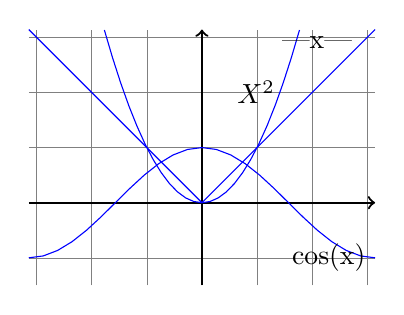
\begin{tikzpicture}[scale = 0.7]
            \draw [help lines] (-pi,-1.5) grid (pi,pi);  %Gitter
            \draw [thick, ->](-pi,0) -- (pi,0);         %x-achse
            \draw [thick, ->](0,-1.5) -- (0,pi);         %y-achse
            \draw [blue, domain=-1.77:1.77] plot (\x, {pow(\x, 2)});
            \node [left] at (1.5,2) {$ X^2$};
            \draw [blue, domain=-pi:pi] plot (\x, {cos(\x r)});
            \node [left] at (pi,-1) {cos(x)};
            \draw [blue, domain=-pi:pi] plot (\x, {abs(\x});
            \node [left] at (2.9,2.9) {|x|};
        \end{tikzpicture}

    \end{minipage}
                
    \begin{minipage}{\linewidth}
        \textbf{Ungerade}\newline
        $f(-t) = -f(t)$ \newline
        Punktsymetrisch am Ursprung
        \[  a_{n} = 0, b_{n} = \frac{4}{T}\int\limits_{0}^{\frac{T}{2}} f(t) \cdot sin(n \omega t)\diff t \]
        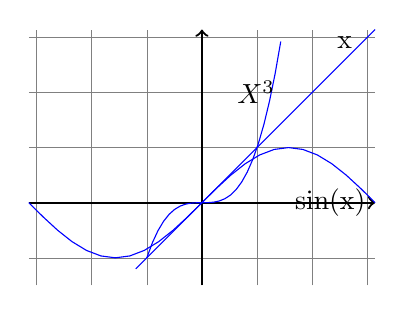
\begin{tikzpicture}[scale = 0.7]
            \draw [help lines] (-pi,-1.5) grid (pi,pi);  %Gitter
            \draw [thick, ->](-pi,0) -- (pi,0);         %x-achse
            \draw [thick, ->](0,-1.5) -- (0,pi);         %y-achse
            \draw [blue, domain=-1:1.43] plot (\x, {pow(\x, 3)});
            \node [left] at (1.5,2) {$ X^3$};
            \draw [blue, domain=-pi:pi] plot (\x, {sin(\x r)});
            \node [left] at (pi,0) {sin(x)};
            \draw [blue, domain= -1.2:pi] plot (\x, {\x});
            \node [left] at (2.9,2.9) {x};
        \end{tikzpicture}

\end{minipage}
\end{multicols}
\clearpage

\section{Lösen von Differentialgleichungen}
\subsection{Allgemeine Vorgehensweisen}
\subsubsection{Trennung von Variablen / Separation}

\begin{tabular}{p{4cm}p{10.5cm}}
\textbf{Form:} $y' = f(x) g(y)$ &
\textbf{Vorgehen:}
\begin{enumerate}
	\item DGL umstellen: $\frac{y'}{g(y)} = f(x)$
	\item Beidseitig nach x integrieren wobei $dx = \frac{dy}{y'}$
	\item Grenzen anpassen: $\int\limits_{y_0=y(x_0)}^{y} \frac{1}{g(y)} dy = \int\limits_{x}^{x_0}f(x) dx$
\end{enumerate}
\end{tabular}
            
\subsubsection{Lineartermsubstitution}

\begin{tabular}{p{5cm}p{10.5cm}}
\textbf{Form:} $y'=f(ax+by+c)$   &
\textbf{Vorgehen:}
\begin{enumerate}
	\item Substitution: $z=ax+by+c$
	\item Einsetzen in $z'=a+bf(z)$
	\item Separation: $\frac{z'}{f(z)} = a + b$ wobei $z_0 = x_0 + y_0$
\end{enumerate}
\end{tabular}
                
\subsubsection{Gleichgradigkeit}
\begin{tabular}{p{4cm}p{10.5cm}}
\textbf{Form:} $y'=f(\frac{y}{x})$ &
\textbf{Vorgehen:}
\begin{enumerate}
	\item Substitution:\quad $z=\frac{y}{x}$
	\item Einsetzen in $z'=\frac{1}{x}(f(z)-z)$
	\item Separation: $\frac{z'}{f(z)-z} = \frac{1}{x}$ wobei $z_0 = \frac{y_0}{x_0}$ 
\end{enumerate}
\end{tabular}
            
\subsection{Differentialgleichung 1. Ordnung}
    
\subsubsection{Konstante Störung $f(x) = A$}
\begin{enumerate}
	\item Homogene Lösung mit $y_h = 0$ berechnen
	
	\item Partikuläre Lösung mit $y_p = B$ (= Konstante) berechnen, indem zeitlich abhängige Terme der DGL ignoriert werden
\end{enumerate}

\subsubsection{Sinusförmige Störung $f(x) = (A \cdot \cos \omega x + B \cdot \sin \omega x)$}
\begin{enumerate}
	\item Homogene Lösung mit $y_h = 0$ berechnen
	
	\item Ansatz für Partikuläre Lösung: $y_p = C \cdot \sin(\omega t) + D\cdot \cos(\omega t)$
	
	\item $y_p$ in DGL einsetzen, $C$ und $D$ per Koeffizientenvergleich ermitteln
\end{enumerate}

\subsection{Störgliedtabelle}
\begin{tabular}{|p{8cm}|p{10cm}|}
    \hline 	
    Störglied $g(x)$ & Ansatz $y_p$ \\
    \hline
    $k$ (Konstante) & $A$ \\
    \hline
    $x^n$ & \multirow{2}{*}{$A_n*x^n + \dots + A_1*x + A_0$} \\
    $p_n(x) = b_n*x^n + \dots + b_1*x + b_0$ & \\
    \hline
    $k*e^{m*x}$ & $A*e^{m*x}$ \\
    \hline	
    $k*cos(b*x)$ & \multirow{3}{*}{$A*cos(b*x) + B*sin(b*x)$} \\
    $k*sin(b*x)$ & \\
    $k_1*cos(b*x) + k_2*sin(b*x)$ & \\
    \hline
    $k*e^{m*x}*cos(b*x)$ & \multirow{3}{*}{$e^{m*x}*(A*cos(b*x) + B*sin(b*x))$} \\
    $k*e^{m*x}*sin(b*x)$ & \\
    $e^{m*x}*(k_1*cos(b*x) + k_2*sin(b*x)$ & \\
    \hline
    $k*cosh(b*x)$ & \multirow{3}{*}{$A*cosh(b*x) + B*sinh(b*x)$} \\
    $k*sinh(b*x)$ & \\
    $k_1*cosh(b*x) + k_2*sinh(b*x)$ & \\
    \hline
    $k*e^{m*x}*cosh(b*x)$ & \multirow{3}{*}{$e^{m*x}*(A*cohs(b*x) + B*sinh(b*x))$} \\
    $k*e^{m*x}*sinh(b*x)$ & \\
    $e^{m*x}*(k_1*cosh(b*x) + k_2*sinh(b*x)$ & \\
    \hline
    $k*x*e^{mx}$ & $(A*x+B)*e^{m*x}$ \\
    \hline
    $p_n(x)*e^{m*x}$ & $(A_n*x^n + \dots + A_1*x + A_0)*e^{mx}$ \\
    \hline
    $x*(k_1*cos(b*x) + k_2*sin(b*x))$ & $(A_1*x+B_1)*cos(b*x) + (A_2*x+B_2)*sin(b*x)$ \\
    \hline
    $x*e^{mx}*(k_1*cos(b*x) + k_2*sin(b*x))$ & $e^{mx}*((A_1*x+B_1)*cos(b*x) + (A_2*x+B_2)*sin(b*x))$ \\
    \hline
    $x*(k_1*cosh(b*x) + k_2*sinh(b*x))$ & $(A_1*x+B_1)*cosh(b*x) + (A_2*x+B_2)*sinh(b*x)$ \\
    \hline
    $x*e^{mx}*(k_1*cosh(b*x) + k_2*sinh(b*x))$ & $e^{mx}*((A_1*x+B_1)*cosh(b*x) + (A_2*x+B_2)*sinh(b*x))$ \\
    \hline
\end{tabular}
\clearpage
\input{idiotenseite/IdiotenseiteInclude}
\pagebreak
%\section{Glossar}
\begin{tabular}{ll}
    GTO & Gate Turn-Off Thyristor \\ 
    IGCT& Integrated Gate-Commutated Thyristor \\ 
    BT  & Bipolarer Transistor  \\ 
    MOS & Metal Oxide Semiconductor \\ 
    IGBT& Insulated-Gate Bipolar Transistor \\ 
\end{tabular} 
\end{document}
